% !TEX root = ./main.tex


%-----------------------------------------------------------------------------
%    STARTER
%-----------------------------------------------------------------------------

\documentclass{backend/backend}
\usepackage{backend/font}
\usepackage{backend/colors}
\usepackage{backend/structure}
\usepackage{backend/informations}

%-----------------------------------------------------------------------------
%    PRESENTATION SLIDES
%-----------------------------------------------------------------------------

\begin{document}
\justifying

\begin{frame}
    \titlepage
\end{frame}

% \comment{  %%%%%%%%%%%%%%%%%%%%%%%%%%%%%%%%%%%%% COMMENTARY
% } %%%%%%%%%%%%%%%%%%%%%%%%%%%%%%%%%%%%% COMMENTARY


\section*{Introduction}
\showtoctrue % active l'affichage des slides de transition

\begin{frame}{Introduction - 1}
    \pause
    \begin{exampleblock}{HACL*}
        \textit{"\textbf{H}igh \textbf{A}ssurance \textbf{C}ryptography \textbf{L}ibrary"}\cite{HACL*}\footnote{\url{https://hacl-star.github.io/}} est une bibliothèque cryptographique, écrite en F* ("F star"), implémentant tous les algorithmes de cryptographie modernes et est prouvée mathématiquement sûre. 
        \smallbreak
        HACL* est notamment utilisé dans plusieurs systèmes de production tels que Mozilla Firefox, le noyau Linux, le VPN WireGuard...
    \end{exampleblock}
\end{frame}

\begin{frame}{Introduction - 2}
    \begin{block}{1996 : Paul C. Kocher, \textit{Timing Attacks on Implementations of Diffie-Hellman, RSA, DSS, and Other Systems} }
        Une mesure précise du temps requis par des opérations sur les clés secrètes permettrait à un attaquant de casser le cryptosystème.
    \end{block}
    \pause
    2003 : \citeauthor{270176} \citetitle{270176}\\
    \pause
    2011 : \citeauthor{stillPractical} \citetitle{stillPractical}
\end{frame}


\begin{frame}{Introduction - 3}
    \begin{enumerate}
        \item[\textbf{QR1}] Est-il possible de propager les garanties de sécurité pendant la compilation ?
        \item[\textbf{QR2}] Est-il possible d'automatiser la détection de ces failles sur des fichiers compilés ?
        \item[\textbf{QR3}] Est-il possible d'appliquer ces mécanismes pour assurer la vérification d'une bibliothèque cryptographique ?
    \end{enumerate}
\end{frame}

%%%%%%%%%%%%%%%%%%%%%%%%%%%%%%%%%%%%%%%%%
%
%         SUMMARY
%
%%%%%%%%%%%%%%%%%%%%%%%%%%%%%%%%%%%%%%%%%
\begin{frame}{Sommaire}
        \small
        \tableofcontents
\end{frame}


%%%%%%%%%%%%%%%%%%%%%%%%%%%%%%%%%%%%%%%%%
%
%         PREMIERE PARTIE
%
%%%%%%%%%%%%%%%%%%%%%%%%%%%%%%%%%%%%%%%%%
\section{Méthodes de protection et limitations}

\begin{frame}{État des lieux}
    \begin{blockSimple}{Usage sécurisé}
        \centering
        \begin{tikzpicture}[>={Latex[length=3mm,width=2.5mm]}, link/.style={->, very thick}]

        % Nœuds avec apparition progressive
        \node[src] (src) {Source};
        \node[comp, right=18mm of src] (cmp) {Compilateur};
        \node[asm, right=18mm of cmp] (asm) {Assembleur};

        % Flèches
        \draw[link] (src) -- (cmp);
        \draw[link] (cmp) -- (asm);

        \end{tikzpicture}
    \end{blockSimple}
\end{frame}


\begin{frame}{Analyse en remontée - 1}

    \begin{blockSimple}{Écrire en assembleur}
        \begin{columns}
            \begin{column}{0.3\textwidth}
                + Efficace\\
                + Contrôle total
            \end{column}
            \begin{column}{0.5\textwidth}
            - Restreint l'architecture et les usages\\
            - Beaucoup de connaissance spécifique au processeur ciblé
            \end{column}
        \end{columns}        
    \end{blockSimple}

    \vspace{6em}
    \begin{blockSimple}{}
        \centering
        \begin{tikzpicture}[scale=0.5, transform shape,>={Latex[length=3mm,width=2.5mm]}, link/.style={->, very thick}]

        % Nœuds avec apparition progressive
        \node[gray] (src) {Source};
        \node[gray, right=18mm of src] (cmp) {Compilateur};
        \node[asm, right=18mm of cmp] (asm) {Assembleur};

        % Flèches
        \draw[link] (src) -- (cmp);
        \draw[link] (cmp) -- (asm);

        \end{tikzpicture}
    \end{blockSimple}
\end{frame}


\begin{frame}{Analyse en remontée - 2}

    \begin{blockSimple}{Utilisation des compilateurs}
        \begin{columns}
        \begin{column}{0.5\textwidth}
            \begin{itemize}
                \item Constantine - 2021
                \item Jasmin - 2017
                \item \alt<1>{Raccoon - 2015}{\sout{Raccoon} - 2015}
                \item CompCert - 2008 (2019)
            \end{itemize}
        \end{column}
        \begin{column}{0.5\textwidth}
          \onslide<2>{
            \begin{itemize}
            \item[-] Couverture des architectures supportée
            \item[-] Informations à transmettre
            \item[-] Spécifications ne sont plus respectées
            \end{itemize}
          }
        \end{column}
    \end{columns}
    \end{blockSimple}
    \vspace{3em}
    \begin{blockSimple}{}
        \centering
        \begin{tikzpicture}[scale=0.5, transform shape,>={Latex[length=3mm,width=2.5mm]}, link/.style={->, very thick}]

        % Nœuds avec apparition progressive
        \node[gray] (src) {Source};
        \node[comp, right=18mm of src] (cmp) {Compilateur};
        \node[gray, right=18mm of cmp] (asm) {Assembleur};

        % Flèches
        \draw[link] (src) -- (cmp);
        \draw[link] (cmp) -- (asm);

        \end{tikzpicture}
    \end{blockSimple}
\end{frame}

\begin{frame}{Analyse en remontée - 3}

    \begin{blockSimple}{Programmation en temps constant}
        \begin{columns}
            \begin{column}{0.3\textwidth}
                + Position haut niveau\\
                + Couverture d'architectures importantes
            \end{column}
            \begin{column}{0.5\textwidth}
            - Rigueur et conception particulière des actions\\
            - Identification des points de fuites
            \end{column}
        \end{columns}        
    \end{blockSimple}

    \vspace{4em}
    \begin{blockSimple}{}
        \centering
        \begin{tikzpicture}[scale=0.5, transform shape,>={Latex[length=3mm,width=2.5mm]}, link/.style={->, very thick}]

        % Nœuds avec apparition progressive
        \node[src] (src) {Source};
        \node[gray, right=18mm of src] (cmp) {Compilateur};
        \node[gray, right=18mm of cmp] (asm) {Assembleur};

        % Flèches
        \draw[link] (src) -- (cmp);
        \draw[link] (cmp) -- (asm);

        \end{tikzpicture}
    \end{blockSimple}
\end{frame}


\begin{frame}[fragile]{Opérations dangereuses}

    \begin{columns}
        \begin{column}{0.4\textwidth}
            \begin{blockSimple}{Opérations influantes :}
                \begin{itemize}
                    \item Accès mémoire
                    \item Décalage/rotation de valeurs \hfill\onslide<2>{(caché)}
                    \item Saut conditionnel
                    \item Division/multiplication
                \end{itemize}
            \end{blockSimple}
        \end{column}
        \pause
        \begin{column}{0.5\textwidth}
            \begin{minted}[frame=lines,framesep=2mm,baselinestretch=1.2,fontsize=\tiny,linenos, gobble=8]{C}
                bool check_pwd(msg, pwd){
                if (msg.length != pwd.length){
                    return False
                }
                for(int i = 0; i < msg.length; i++){
                    if(msg[i] != pwd[i]){
                        return False
                    }
                }
                return True
                }
            \end{minted}
            \begin{tikzpicture}[scale = 0.5, transform shape]
            % Noeuds
            \node (start) [startstop] {check\_pwd};
            \node (valid) [right of=start, xshift=9cm, green] {\huge{$\checkmark$}};
            \draw [arrow] (start) -- (valid);
            
            \node (inputs) [below of = start, yshift=0.2cm] {(msg, pwd)};
            \node (if) [process] [right of=start, xshift=2cm] {if};
            \node (not) [above of=if, red] {\huge{$\times$}};
            \node (for) [process] [right of=if,, xshift=2cm] {for};
            \node (for1) [above of=for,xshift=1cm, red] {\huge{$\times$}};
            \node (for2) [right of=for1, red] {\huge{$\times$}};
            \node (for3) [right of=for2, red] {\huge{$\times$}};

            \draw [arrow] (if) -- (not);
            \draw [arrow] (for) -- (for1);
            \draw [arrow] (for) -- (for2);
            \draw [arrow] (for) -- (for3);

            \node (t) [above of=start] {};
            \node (a) [above of=valid, xshift=-0.3cm] {};
            \draw [arrow] (t) -- node[above left] {Temps ($\mu$s)} (a.west);
            
            \end{tikzpicture}
        \end{column}
    \end{columns}

\end{frame}

\begin{frame}{Plus de problème ?}
    \pause
    \begin{blockSimple}{Mauvaises nouvelles \alt<2>{?}{!}}
        2019 : \citeauthor{binsecRel2019}, \citetitle{binsecRel2019}\\
        \pause
        2024 : \citeauthor{schneider2024breakingbadcompilersbreak}, \citetitle{schneider2024breakingbadcompilersbreak}
    \end{blockSimple}
\end{frame}

%%%%%%%%%%%%%%%%%%%%%%%%%%%%%%%%%%%%%%%%%
%
%         DEUXIEME PARTIE
%
%%%%%%%%%%%%%%%%%%%%%%%%%%%%%%%%%%%%%%%%%

\section{Outils de vérifications}
\begin{frame}{Spécialisations}
    \begin{columns}% t = alignement en haut
    % Colonne gauche : tableau
    \column{0.6\textwidth}
    \tiny
    \begin{tabular}{lccc}
        \toprule
        \textbf{Outil} & \textbf{Cible} & \textbf{Techn.} & \textbf{Garanties} \\
        \rowcolor{lightgray}
        ctgrind \cite{ctgrind} & Binaire & Dynamique & $\blacktriangle$ \\
        ABPV13 \cite{ABPV13} & C & Formel & $\bullet$ \\
        \rowcolor{lightgray}
        VirtualCert \cite{VirtualCert} & x86 & Formel & $\bullet$ \\
        ct-verif \cite{ctverif} & LLVM & Formel & $\bullet$ \\
        \rowcolor{lightgray}
        FlowTracker \cite{FlowTracker} & LLVM & Formel & $\bullet$ \\
        Blazer \cite{Blazer} & Java & Formel & $\bullet$ \\
        \rowcolor{lightgray}
        BPT17 \cite{BPT17} & C & Symbolique & $\blacktriangle$ \\
        MemSan \cite{MemSan} & LLVM & Dynamique & $\blacktriangle$ \\
        \rowcolor{lightgray}
        Themis \cite{Themis} & Java & Formel & $\bullet$ \\
        COCO-CHANNEL \cite{COCOCHANNEL} & Java & Symbolique & $\bullet$ \\
        \rowcolor{lightgray}
        DATA \cite{DATA1,DATA2} & Binaire & Dynamique & $\blacktriangle$ \\
        MicroWalk \cite{MicroWalk} & Binaire & Dynamique & $\blacktriangle$ \\
        \rowcolor{lightgray}
        timecop \cite{timecop} & Binaire & Dynamique & $\blacktriangle$ \\
        SC-Eliminator \cite{SCEliminator} & LLVM & Formel & $\bullet$ \\
        \rowcolor{lightgray}
        Binsec/Rel \cite{binsecRel2019} & Binaire & Symbolique & $\blacktriangle$ \\
        CT-WASM \cite{CTWASM} & WASM & Formel & $\bullet$ \\
        \rowcolor{lightgray}
        FaCT \cite{FaCT} & DSL & Formel & $\bullet$ \\
        haybale-pitchfork \cite{haybale-pitchfork} & LLVM & Symbolique & $\blacktriangle$ \\
        \bottomrule
    \end{tabular}

    % Colonne droite : légende et titre
    \column{0.5\textwidth}
    \textbf{Liste d’outils de vérification}\\[1ex]
    Source : \cite{notThatHardCT}\\[2ex]
    \begin{scriptsize}
        
        \textbf{Cible}
        \begin{itemize}
        \item[[C, Java]] Code source
        \item[Binaire] Binaire
        \item[DSL] Surcouche de langage
        \item[Trace] Trace d'exécution
        \item[WASM] Assembleur web
    \end{itemize}
    \textbf{Techn.}
    \begin{itemize}
        \item[Formel] Programmation formelle 
        \item[[*]] type d'analyse
    \end{itemize}
    \textbf{Garanties (attaques temporelles)}\\
        $\bullet$ = Analyse correcte,$\blacktriangle$ =  Limitée
    \end{scriptsize}
    \end{columns}
\end{frame}

\begin{frame}{L'outil idéal}
    \begin{exampleblock}{Binsec}
       \textit{Binary Security}\footnote{\url{https://binsec.github.io/}} est une plateforme open source développée pour évaluer la sécurité des logiciels au niveau binaire. 
       
       Il est notamment utilisé pour la recherche de vulnérabilités, la désobfuscation de logiciels malveillants et la vérification formelle de code binaire. Grâce à l'exécution symbolique, Binsec peut explorer et modéliser le comportement d'un programme pour détecter des erreurs; cette détection est réalisée en association avec des outils de fuzzing et/ou des solveurs SMT.
    \end{exampleblock}
\end{frame}

\section{Automatismes}
\begin{frame}[fragile]{Premiers scripts}

    \textbf{Code :} Instructions permettant de trouver le mot d'un passe d'un binaire d'exercice
    \begin{minted}[frame=lines,framesep=2mm,baselinestretch=1.2,linenos, fontsize=\tiny]{bash}
starting from core with
  argv<64> := rsi
  arg1<64> := @[argv + 8, 8]
  size<64> := nondet            # 0 < strlen(argv[1]) < 128
  assume 0 < size < 128,       all_printables<1> := true
  @[arg1, 128] := 0
  for i<64> in 0 to size - 1 do
    @[arg1 + i] := nondet as password
    all_printables := all_printables && " " <= password <= "~"
  end
  assume all_printables
end

replace <puts>, <printf> by return end

reach <puts> such that @[rdi, 14] = "Good password!"
then print ascii stream password

cut at <puts> if @[rdi, 17] = "Invalid password!"
halt at <printf>
\end{minted}


\end{frame}

\begin{frame}[fragile]{Simplification}
\textbf{Codes :} Instructions permettant d'analyser le code précédent compilé vers Risc-V 32bits
    
\begin{minted}[frame=lines,framesep=2mm,baselinestretch=1.2,linenos,fontsize=\scriptsize]{C}
#include <stdlib.h>
#include <stdint.h>
#include "Hacl_P256.h"

#define SIZE 4
uint64_t cin;
uint64_t x[SIZE]; uint64_t y[SIZE]; uint64_t r[SIZE];

int main(){
  bn_cmovznz4(r, cin, x, y);
}
\end{minted}
\end{frame}

\begin{frame}[fragile]{Adaptation}
    \textbf{Codes :} Instructions permettant d'analyser le code précédent compilé vers Risc-V 32bits
    
    \begin{minted}[frame=lines,framesep=2mm,baselinestretch=1.2,linenos]{bash}
load sections .plt, .text, .rodata, .data, .got, .got.plt, .bss from file

secret global  r, cin, y, x

starting from <main>

with concrete stack pointer
halt at  0x0000000000000464
explore all

\end{minted}
\end{frame}

\begin{frame}{Premiers pas vers l'automatisation}
    
    \textbf{Table :} Tableau de résultats d'analyse Binsec pour architecture ARMv7 et ARMv8
    \begin{center}    
        \begin{tabular}{|c|c|c|c|c|c|}
            \hline
            \rowcolor{blue!10}
            \cellcolor{inria-2024-gris-bleu!20}\textbf{opt}\textbackslash\textbf{fonction analysée} & \multicolumn{5}{c|}{\textbf{cmovznz4}} \\
            \hline
            \rowcolor{blue!30}
            \textbf{Clang+LLVM} & \textbf{14.0.6} & \textbf{15.0.6} & \textbf{16.0.4} & \textbf{17.0.6} & \textbf{18.1.8} \\
            \hline
            \rowcolor{orange!30!red!50}
            \textbf{-O0} & \cellcolor{green!60}\checkmark & \cellcolor{green!60}\checkmark & \cellcolor{green!60}\checkmark  & \cellcolor{green!60}\checkmark  & \cellcolor{green!60}\checkmark  \\
            \hline
            \rowcolor{orange!30!red!50}
            \textbf{-O1} & \cellcolor{green!60}\checkmark & \cellcolor{green!60}\checkmark & \cellcolor{green!60}\checkmark  & \cellcolor{green!60}\checkmark  & \cellcolor{green!60}\checkmark  \\
            \hline
            \rowcolor{orange!30!red!50}
            \textbf{-O2} & \cellcolor{green!60}\checkmark & \cellcolor{green!60}\checkmark & \cellcolor{green!60}\checkmark  & \cellcolor{green!60}\checkmark  & \cellcolor{green!60}\checkmark  \\
            \hline
            \rowcolor{orange!30!red!50}
            \textbf{-O3} & \cellcolor{green!60}\checkmark & \cellcolor{green!60}\checkmark  & \cellcolor{green!60}\checkmark  & \cellcolor{green!60}\checkmark  & \cellcolor{green!60}\checkmark  \\
            \hline
            \rowcolor{orange!30!red!50}
            \textbf{-Os} & \cellcolor{green!60}\checkmark  & \cellcolor{green!60}\checkmark  & \cellcolor{green!60}\checkmark  & \cellcolor{green!60}\checkmark  & \cellcolor{green!60}\checkmark  \\
            \hline
            \rowcolor{orange!30!red!50}
            \textbf{-Oz} & \cellcolor{green!60}\checkmark  & \cellcolor{green!60}\checkmark  &  \cellcolor{green!60}\checkmark  &  \cellcolor{green!60}\checkmark  &  \cellcolor{green!60}\checkmark \\
            \hline
        \end{tabular}   
    \end{center}
    \raggedleft
     \small{
        \checkmark : \textit{binary secure} ;
        \textasciitilde : \textit{binary unknown} ;
        $\times$ : \textit{binary insecure}
    }
\end{frame}

\begin{frame}{Reherche de failles}
    \textbf{Table :} Tableau de résultats d'analyse Binsec pour architecture Risc-V
    \begin{center}
    \begin{tabular}{|c|cc|cc|}
        \hline
        \rowcolor{blue!10}
        \cellcolor{inria-2024-gris-bleu!20}\textbf{opt}\textbackslash\textbf{fonction analysée} & \multicolumn{2}{c|}{\textbf{cmovznz4} - 64 bits} & \multicolumn{2}{c|}{\textbf{cmovznz4} - 32 bits} \\
        \hline
        \rowcolor{blue!30}
        \textbf{Compilateur et architecture} & gcc 15.1.0 & clang 19.1.7 & gcc 15.1.0& clang 19.1.7 \\
        \hline
        \rowcolor{orange!30!red!50}
        \textbf{-O0} &  \cellcolor{orange!60}\textasciitilde  & \cellcolor{red!60}$\times$ & \cellcolor{orange!60}\textasciitilde & \cellcolor{red!60}$\times$ \\
        \hline
        \rowcolor{orange!30!red!50}
        \textbf{-O1} &  \cellcolor{green!60}\checkmark & \cellcolor{red!60}$\times$ & \cellcolor{green!60}\checkmark & \cellcolor{red!60}$\times$ \\
        \hline
        \rowcolor{orange!30!red!50}
        \textbf{-O2} &  \cellcolor{green!60}\checkmark & \cellcolor{red!60}$\times$ & \cellcolor{green!60}\checkmark & \cellcolor{red!60}$\times$ \\
        \hline
        \rowcolor{orange!30!red!50}
        \textbf{-O3} &  \cellcolor{green!60}\checkmark & \cellcolor{red!60}$\times$ & \cellcolor{green!60}\checkmark & \cellcolor{red!60}$\times$ \\
        \hline
        \rowcolor{orange!30!red!50}
        \textbf{-Os} &  \cellcolor{green!60}\checkmark & \cellcolor{red!60}$\times$ & \cellcolor{green!60}\checkmark & \cellcolor{red!60}$\times$ \\
        \hline
        \rowcolor{orange!30!red!50}
        \textbf{-Oz} &  \cellcolor{green!60}\checkmark & \cellcolor{red!60}$\times$ & \cellcolor{green!60}\checkmark & \cellcolor{red!60}$\times$ \\
        \hline
    \end{tabular}
    \end{center}
\raggedleft
     \small{
        \checkmark : \textit{binary secure} ;
        \textasciitilde : \textit{binary unknown} ;
        $\times$ : \textit{binary insecure}
    }
\end{frame}

\begin{frame}{Cahier des charges}
\begin{columns}
    \column{0.3\textwidth}
    \begin{blockSimple}{Objectifs du futur outil}
        \begin{itemize}
            \item Petits fichiers binaire
            \item Analyse complète de la bibliothèque
            \item Analyse correcte
            \item Automatique
            \pause
            \item Couverture [architectures, compilateurs] 
        \end{itemize}
    \end{blockSimple}
    \column{0.5\textwidth}
    \textbf{Figure :} Flot de travail de l'outil
    \smallbreak
    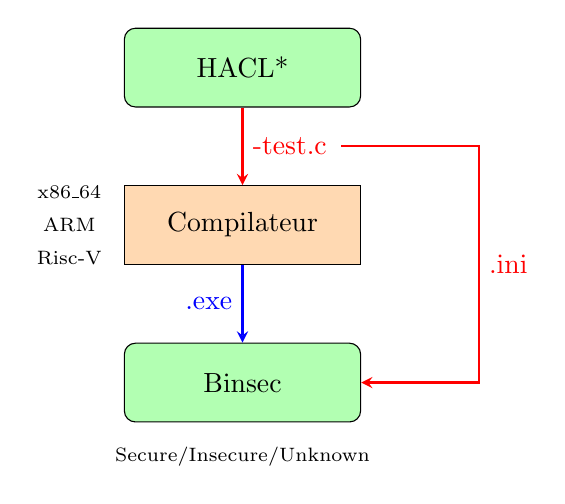
\begin{tikzpicture}[node distance=2cm, scale=1, transform shape]

    % Styles des noeuds
    \tikzstyle{startstop} = [rectangle, rounded corners, minimum width=3cm, minimum height=1cm,text centered, draw=black, fill=green!30]
    \tikzstyle{process} = [rectangle, minimum width=3cm, minimum height=1cm, text centered, draw=black, fill=orange!30]
    \tikzstyle{intermediate} = [circle, minimum size=0.5cm, text centered, draw=white, fill=white]
    \tikzstyle{arrow} = [thick,->,>=stealth]
    
    % Noeuds
    \node (hacl) [startstop] {HACL*};
    \node (inter) [intermediate, below of=hacl,xshift=1cm, yshift=1cm] {};
    \node (compilateur) [process, below of=hacl] {Compilateur};
    \node (binsec) [startstop, below of=compilateur] {Binsec};
    
    % Flèches
    \draw [arrow, red] (hacl) -- node[anchor=west] {-test.c} (compilateur);
    \draw [arrow, red] (inter) -- ++(2,0) |- node[anchor=west, pos=0.25] {.ini} (binsec);
    \draw [arrow, blue] (compilateur) -- node[anchor=east] {.exe} (binsec);
    
    % Annotations
    \node[align=center, left of=compilateur, xshift=-0.2cm] {\scriptsize x86\_64\\ \scriptsize ARM\\ \scriptsize Risc-V};
    \node[align=center, below of=binsec, yshift=30pt] {\scriptsize Secure/Insecure/Unknown};
    
    \end{tikzpicture}
\end{columns}
\end{frame}



\section{Érysichthon}
\subsection{Conception générale}

\begin{frame}{Conception générale}
    \begin{center}
        \begin{tikzpicture}[remember picture, overlay]
            \begin{scope}[shift={([yshift=-2.3cm, xshift=-1cm]current page.north)}]
    % Styles
    \tikzstyle{startstop} = [rectangle, rounded corners, minimum width=2cm, minimum height=1cm, text centered, draw=black, fill=green!30]
    \tikzstyle{process} = [rectangle, minimum width=2cm, minimum height=1cm, text centered, draw=black, fill=orange!30]
    \tikzstyle{arrow} = [thick,->,>=stealth]
    \tikzset{zone1/.style={rectangle, rounded corners, draw=red, dashed, fill=red!10, inner sep=0.3cm}}
    \tikzset{zone2/.style={rectangle, rounded corners, draw=blue, dashed, fill=blue!10, inner sep=0.3cm, opacity = 0.5}}
    \tikzset{zone3/.style={rectangle, rounded corners, draw=green, dashed, fill=green!10, inner sep=0.3cm}}
    
    % Noeuds
    \node (hacl) [startstop] {HACL*};
    \node (c) [below of=hacl] {Fonction};
    \node (ini) [below of=c] {.ini};
    \node (test) [below of=c, xshift=-2cm] {-test.c};
    \node (compilateur) [process, below of=test] {Compilateur};
    \node (exe) [below of=compilateur] {-test.exe};
    \node (blanc) [below of=c] {};
    \node (blanc1) [below of=blanc] {};
    \node (blanc2) [below of=blanc1] {};
    \node (binsec) [startstop, below of=blanc2] {Binsec};
    
    % Flèches
    \draw [arrow] (hacl) -- (c);
    \draw [arrow] (c) -- (ini);
    \draw [arrow] (c) -- (test);
    \draw [arrow] (test) -- (compilateur);
    \draw [arrow] (compilateur) -- (exe);
    \draw [arrow] (exe) -- (binsec);
    \draw [arrow] (ini) -- (binsec);

    % Zones
    \begin{scope}[on background layer]
        \node [zone1, fit=(c) (ini) (test) ] {};
        \node [zone2, fit=(ini) (binsec)] {};
        \node [zone3, fit=(compilateur) (exe)] {};
    \end{scope}
    \end{scope}




        \node[anchor=north east] at ([xshift=-5mm,yshift=-3cm]current page.north east) {
    \begin{tikzpicture}[font=\small]
    \node[rectangle, draw=black, fill=white, rounded corners, inner sep=2mm] {
        \begin{tabular}{l}
        \textbf{Légende :} \\
        \textcolor{red}{\rule{0.5cm}{0.3cm}} Difficile \\
        \textcolor{blue}{\rule{0.5cm}{0.3cm}} Relativement simple \\
        \textcolor{green}{\rule{0.5cm}{0.3cm}} Simple
        \end{tabular}
    };
\end{tikzpicture}
};
    \end{tikzpicture}
    \end{center}
\end{frame}

\begin{frame}{Adaptation architecturale}
    \begin{tikzpicture}[remember picture, overlay]
    \begin{scope}[shift={([yshift=-2.3cm, xshift=-3cm]current page.north)}]
    % Styles
    \tikzstyle{startstop} = [rectangle, rounded corners, minimum width=2cm, minimum height=1cm, text centered, draw=black, fill=green!30]
    \tikzstyle{process} = [rectangle, minimum width=2cm, minimum height=1cm, text centered, draw=black, fill=orange!30]
    \tikzstyle{arrow} = [thick,->,>=stealth]
    \tikzset{zone1/.style={rectangle, rounded corners, draw=red, dashed, fill=red!10, inner sep=0.3cm}}
    \tikzset{zone2/.style={rectangle, rounded corners, draw=blue, dashed, fill=blue!10, inner sep=0.3cm, opacity = 0.7}}
    \tikzset{zone22/.style={rectangle, rounded corners, draw=none, fill=blue!10, inner sep=0.3cm}}
    \tikzset{zone3/.style={rectangle, rounded corners, draw=green, dashed, fill=green!10, inner sep=0.3cm}}
    
    % Noeuds
    \node (hacl) [startstop] {HACL*};
    \node (c) [below of=hacl] {Fonction};
    \node (ini) [below of=c, xshift=2cm] {.ini};
    \node (test) [below of=c, xshift=-2cm] {-test.c};
    \node (script) [below of=c] {.script};
    \node (compilateur) [process, below of=test] {Compilateur};
    \node (exe) [below of=compilateur] {-test.exe};
    \node (blanc1) [below of=script] {};
    \node (blanc2) [below of=blanc1] {};
    \node (gdb) [process, below of=blanc2] {GDB};
    \node (snap) [right of=gdb, xshift=2cm] {.snapshot};
    \node (binsec) [startstop, right of=snap, xshift=1.5cm] {Binsec};
    
    % Flèches
    \draw [arrow] (hacl) -- (c);
    \draw [arrow] (c) -- (ini);
    \draw [arrow] (c) -- (test);
    \draw [arrow] (c) -- (script);
    \draw [arrow] (test) -- (compilateur);
    \draw [arrow] (compilateur) -- (exe);
    \draw [arrow] (exe) -- (gdb);
    \draw [arrow] (script) -- (gdb);
    \draw [arrow] (gdb) -- (snap);
    \draw [arrow] (snap) -- (binsec);
    \draw [arrow] (ini) -- (binsec);

    % Zones
    \begin{scope}[on background layer]
        \node [zone1, fit=(c) (ini) (test) (script)] {};
        \node [zone2, fit=(script) (gdb)] {};
              \node [zone2, fit=(gdb) (snap) (binsec)] {};
              \draw [zone22]
              ([xshift=-10pt, yshift=10pt]gdb.north west) --
              ([xshift=10pt, yshift=10pt]gdb.north east) -- 
              ([xshift=10pt, yshift=-9pt]gdb.south east) -- 
              ([xshift=1pt, yshift=-1pt]gdb.south west) --
              cycle;  
    \node [zone3, fit=(compilateur) (exe)] {};
    \end{scope}
\end{scope}
    \node[anchor=north east] at ([xshift=-5mm,yshift=-3cm]current page.north east) {
    \begin{tikzpicture}[font=\small]
    \node[rectangle, draw=black, fill=white, rounded corners, inner sep=2mm] {
        \begin{tabular}{l}
        \textbf{Légende :} \\
        \textcolor{red}{\rule{0.5cm}{0.3cm}} Difficile \\
        \textcolor{blue}{\rule{0.5cm}{0.3cm}} Relativement simple \\
        \textcolor{green}{\rule{0.5cm}{0.3cm}} Simple
        \end{tabular}
    };
\end{tikzpicture}
};
\end{tikzpicture}
\end{frame}

\begin{frame}{Construction en modules}
    \begin{center}
        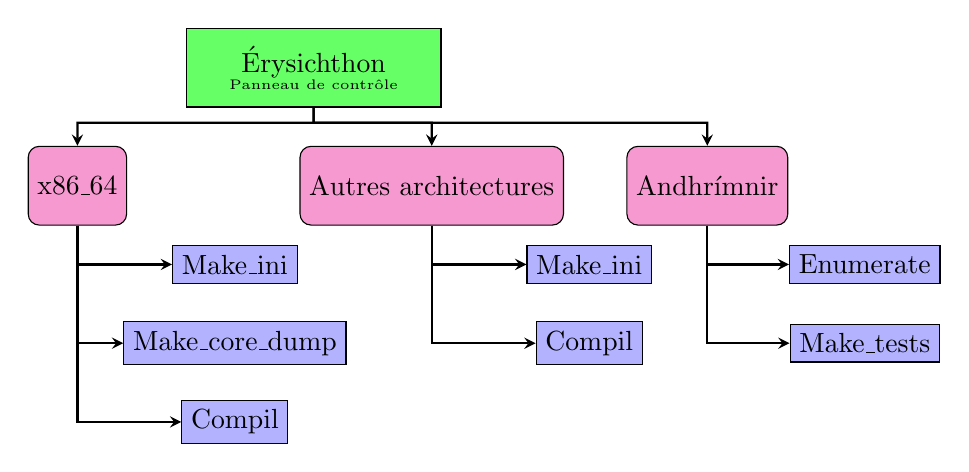
\begin{tikzpicture}[auto]

    % Styles
    \tikzstyle{startstop} = [rectangle, minimum width=2cm, minimum height=1cm, text centered, draw=black, fill=green!60]
    \tikzstyle{process} = [rectangle, rounded corners,minimum width=1cm, minimum height=1cm, text centered, draw=black, fill=magenta!40]
     \tikzstyle{process2} = [rectangle, minimum width=0.8cm, minimum height=0.3cm, text centered, draw=black, fill=blue!30]
    \tikzstyle{arrow} = [thick,->,>=stealth]
    
    % Noeuds
    \node (control) [startstop] {\parbox{3cm}{\centering Érysichthon \\ \tiny{Panneau de contrôle}}};
    \node (x86) [process, below of=control, xshift= -3cm, yshift=-0.5cm] {x86\_64};
    \node (x86-ini) [process2, below of=x86, xshift = 2cm] {Make\_ini};
    \node (x86-dump) [process2, below of=x86-ini] {Make\_core\_dump};
    \node (x86-compil) [process2, below of=x86-dump] {Compil};

    \node (arm) [process, below of=control, xshift = 1.5cm, , yshift=-0.5cm] {Autres architectures};
    \node (arm-ini) [process2, below of=arm, xshift=2cm] {Make\_ini};
    \node (arm-compil) [process2, below of=arm-ini] {Compil};

    \node (test) [process, below of=control, xshift = 5cm, , yshift=-0.5cm] {Andhrímnir};
    \node (enum) [process2, below of=test, xshift=2cm] {Enumerate};
    \node (exe) [process2, below of=enum] {Make\_tests};

    % Flèches
    \draw [arrow] (control) -- ++(0,-0.7) -- ++(-3,0) -- (x86.north);
    \draw [arrow] (control) -- ++(0,-0.7) -- ++(1.5,0) -- (arm.north);
    \draw [arrow] (control) -- ++(0,-0.7) -- ++(5,0) -- (test.north);
    \draw [arrow] (x86) -- ++(0,-1) -- (x86-ini);
    \draw [arrow] (x86) -- ++(0,-2) -- (x86-dump);
    \draw [arrow] (x86) -- ++(0,-3) -- (x86-compil);
    \draw [arrow] (arm) -- ++(0,-1) -- (arm-ini);
    \draw [arrow] (arm) -- ++(0,-2) -- (arm-compil);
    \draw [arrow] (test) -- ++(0,-1) -- (enum);
    \draw [arrow] (test) -- ++(0,-2) -- (exe);
    
    \end{tikzpicture}
    \end{center}
\end{frame}


\subsection{Andhrímnir}

\begin{frame}{Andhrímnir - 1}
    \begin{blockSimple}{Module indépendant}
        \begin{itemize}
            \item Réalise des tests complet d'un projet C
            \item Réalise des tests automatiquement
        \end{itemize}
    \end{blockSimple}
    \pause
    \begin{blockSimple}{Module adapté}
        \begin{itemize}
            \item Optimisation pour HACL*
            \item Communications avec Érysichthon
            \item Adaptées pour de l'analyse symbolique
        \end{itemize}
    \end{blockSimple}
\end{frame}



\begin{frame}[fragile]{Exemple de test}
    \textbf{Code :}Test de la fonction Hacl\_EC\_K256\_felem\_sqr
  \begin{minted}[fontsize=\scriptsize]{c}
// Made by
// ANDHRÍMNIR - 0.3.0
// 09-07-2025
//

#include <stdlib.h>
#include "Hacl_EC_K256.h"

#define BUFFER_SIZE 5
uint64_t a[BUFFER_SIZE];
uint64_t out[BUFFER_SIZE];


int main (int argc, char *argv[]){
Hacl_EC_K256_felem_sqr(a, out);
  exit(0);
}   
  \end{minted}
\onslide<2>{
  \begin{tikzpicture}[overlay , remember picture, node distance=0.5cm]
    
    \tikzset{intro/.style={rectangle, rounded corners, draw=green, fill=green!50, inner sep=0.3cm, opacity=0.2, font=\bfseries}}
    \tikzset{definition/.style={rectangle, rounded corners, draw=blue, fill=blue!50, inner sep=0.3cm, opacity=0.2, font=\bfseries}}
    \tikzset{main/.style={rectangle, rounded corners, draw=orange, fill=orange!50, inner sep=0.3cm, opacity=0.2, font=\bfseries}}
    \tikzset{labelshift/.style={xshift=3cm, yshift=0.5cm}}

    \node[intro, fit={(0.3,4.1) (12.74,5.9)}, label={[labelshift]center:Phase introductive : 8 lignes}]{};
    \node[definition, fit={(0.3,2.3) (12.74,3.5)}, label={[labelshift]center:Phase déclarative}]{};
    \node[main, fit={(0.3,0.8) (12.74,1.7)}, label={[labelshift]center:Phase principale}]{};

  \end{tikzpicture}
}
\end{frame}

\begin{frame}{Andhrímnir - 2}
    \pause
    \begin{tikzpicture}[scale = 0.7, transform shape]
    % Définition des styles pour les boîtes et flèches
    \tikzset{
      box1/.style={rectangle, draw=black, fill=cyan!30, thick, rounded corners, minimum width=2.5cm, minimum height=1cm, align=center},
      box2/.style={rectangle, draw=black, fill=orange!30, thick, rounded corners, minimum width=2.5cm, minimum height=1cm, align=center},
      box3/.style={rectangle, draw=black, fill=yellow!30, thick, rounded corners, minimum width=2.5cm, minimum height=1cm, align=center},
      box4/.style={rectangle, draw=black, fill=green!30, thick, rounded corners, minimum width=2.5cm, minimum height=1cm, align=center},
      box5/.style={rectangle, draw=black, fill=blue!30, thick, rounded corners, minimum width=2.5cm, minimum height=1cm, align=center},
      box6/.style={rectangle, draw=black, fill=magenta!30, thick, rounded corners, minimum width=2.5cm, minimum height=1cm, align=center},
      box65/.style={rectangle, draw=black, fill=magenta!60, thick, rounded corners, minimum width=1.5cm, minimum height=0.6cm, align=center},
      box7/.style={rectangle, draw=black, fill=red!30, thick, rounded corners, minimum width=2.5cm, minimum height=1cm, align=center},
      box8/.style={rectangle, draw=black, fill=blue!45, thick, rounded corners, minimum width=2.5cm, minimum height=1cm, align=center},
      arrow1/.style={->, thick, color=cyan!70!black},
      arrow2/.style={->, thick, color=orange!80!black},
      arrow3/.style={->, thick, color=yellow!80!black},
      arrow4/.style={->, thick, color=green!80!black},
      arrow5/.style={->, thick, color=blue!80!black},
      arrow6/.style={->, thick, color=magenta!80!black},
      arrow7/.style={->, thick, color=red!80!black},
      arrow8/.style={->, thick, color=gray!80!black}
      }
      \tikzset{zone1/.style={rectangle, rounded corners, draw=blue, dashed, fill=blue!10, inner sep=0.5cm, text width=3cm}}

    % Noeuds principaux (ligne du haut)
    \node[] (build_test) at (0,0) {};
    \node[box2, below of=build_test] (parse_h) {Lecture du .h};
    \node[box3, right=1cm of parse_h] (read_json) {Lecture .json};
    \node[box4, right=1cm of read_json] (build_local_json) {Accumulation d'informations};

    % Ligne du bas (génération du .c)
    \node[box5, below=1cm of build_local_json] (build_intro) {Gen. introduction};
    \node[box6, left=1cm of build_intro] (build_def) {Gen. déclaration};
    \node[box7, left=1cm of build_def] (add_main) {Gen. main};
    \node[box8, left=1cm of add_main] (fichier_c) {fichier .c};

    % Flèches horizontales principales
    \draw[arrow1] (build_test) -- (0,0.6) -- (parse_h);
    \draw[arrow2] (parse_h) -- (read_json);
    \draw[arrow3] (read_json) -- (build_local_json);
    \draw[arrow4] (build_local_json) -- (build_intro);
    \draw[arrow5] (build_intro) -- (build_def);
    \draw[arrow6] (build_def) -- (add_main);
    \draw[arrow7] (add_main) -- (fichier_c);

    % Branche auxiliaire depuis build introduction
    \node[box5, left of = build_intro, yshift=-1cm] (detect_aux) {Détection appel auxiliaire};
    % Ajout de deux barres obliques sur la flèche build_intro -> build_def
    \draw[thick] ($(build_intro)!0.5!(build_def) + (0,0.3)$) -- ($(build_intro)!0.5!(build_def) + (0,-0.54)$);
    \draw[thick] ($(build_intro)!0.55!(build_def) + (0,0.3)$) -- ($(build_intro)!0.55!(build_def) + (0,-0.54)$);


    \node[box3, left=1cm of detect_aux, yshift=-2cm] (test_exist) {test si fichier existe};
    \draw[arrow5] (detect_aux) -- (test_exist);

    % Oui -> Collage -> build definition
    \node[box4, above of = test_exist, yshift=0.5cm] (collage) {\footnotesize{Collage}};
    \draw[->, thick, color=green!80!black] (test_exist) -- node[left, font=\scriptsize] {Oui} (collage);
    \draw[arrow6] (collage) -- (build_def);

    % Non -> Stocker dans liste_temporisée
    \node[box2, left=0.8cm of test_exist, yshift=-0.8cm] (liste_temp) {Stocker dans liste\_temporisée};
    \draw[arrow7] (test_exist) -- node[above,font=\scriptsize] {Non} (liste_temp.east);

    \draw [arrow5, dashed] (liste_temp.east) to[out=-30, in=-30] node[black, below, yshift=-0.5cm] {\textit{Recommence le procédé}} (build_intro.east);

    \begin{scope}[on background layer]
      \node (zoneNode) [zone1, fit=(parse_h) (read_json) (build_local_json) (build_intro) (build_def) (add_main) (fichier_c) (test_exist) (liste_temp) (collage) (detect_aux) (build_test)] {};
        \node (title) [anchor=north west] at (zoneNode.north west) {\parbox{3.5cm}{\centering \Huge{\textbf{Andhrímnir}}\\\scriptsize{\textit{Génère les tests}}}};
    \end{scope}
  \end{tikzpicture}
\end{frame}

\section{Résultats}
\begin{frame}{Premières passes}
    \begin{center}
        \textbf{Graphe :} Résultats d'Érysichthon en x86\_64
    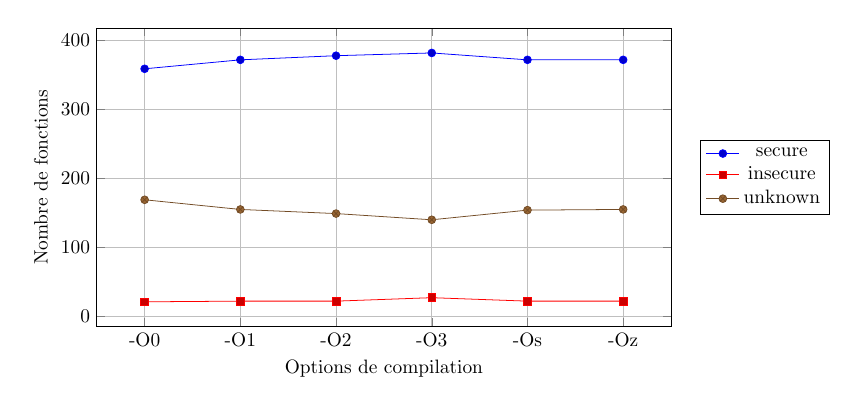
\begin{tikzpicture}[scale = 0.7, transform shape]
      \begin{axis}[
        xlabel={Options de compilation},
        ylabel={Nombre de fonctions},
        legend style={at={(0.5,-0.15)},anchor=north,legend columns=-1},
        grid=both,
        xtick={0,1,2,3,4,5},
        xticklabels={-O0, -O1, -O2, -O3, -Os, -Oz},
        width=12cm, height=7cm,
        legend style={at={(1.05,0.5)}, anchor=west},
        legend columns=1
      ]

        \addplot coordinates {(0,359) (1,372) (2,378) (3,382) (4,372) (5,372)};
        \addlegendentry{secure}

        \addplot coordinates {(0,21) (1,22) (2,22) (3,27) (4,22) (5,22)};
        \addlegendentry{insecure}

        \addplot coordinates {(0,169) (1,155) (2,149) (3,140) (4,154) (5,155)};
        \addlegendentry{unknown}

      \end{axis}
    \end{tikzpicture}%
    \end{center}
\end{frame}

\begin{frame}{Analyses}
    \centering
    \textbf{Graphes :} Détail des erreurs interrompant l'analyse Binsec
    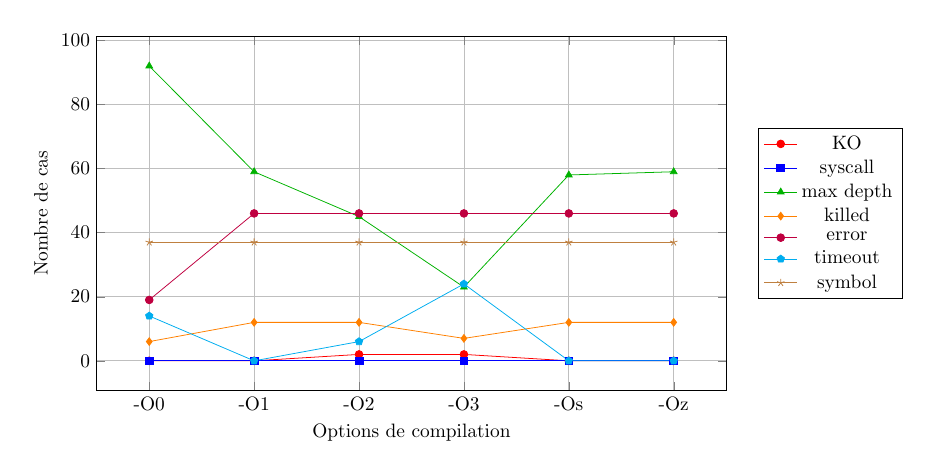
\begin{tikzpicture}[scale = 0.7, transform shape]
  \begin{axis}[
    xlabel={Options de compilation},
    ylabel={Nombre de cas},
    grid=both,
    xtick={0,1,2,3,4,5},
    xticklabels={-O0, -O1, -O2, -O3, -Os, -Oz},
    width=13cm, height=8cm,
    legend style={at={(1.05,0.5)}, anchor=west}
  ]

    % KO
    \addplot[color=red, mark=*] coordinates {(0,0) (1,0) (2,2) (3,2) (4,0) (5,0)};
    \addlegendentry{KO}

    % syscall
    \addplot[color=blue, mark=square*] coordinates {(0,0) (1,0) (2,0) (3,0) (4,0) (5,0)};
    \addlegendentry{syscall}

    % max depth
    \addplot[color=green!70!black, mark=triangle*] coordinates {(0,92) (1,59) (2,45) (3,23) (4,58) (5,59)};
    \addlegendentry{max depth}

    % killed
    \addplot[color=orange, mark=diamond*] coordinates {(0,6) (1,12) (2,12) (3,7) (4,12) (5,12)};
    \addlegendentry{killed}

    % error
    \addplot[color=purple, mark=otimes*] coordinates {(0,19) (1,46) (2,46) (3,46) (4,46) (5,46)};
    \addlegendentry{error}

    % timeout
    \addplot[color=cyan, mark=pentagon*] coordinates {(0,14) (1,0) (2,6) (3,24) (4,0) (5,0)};
    \addlegendentry{timeout}

    % symbol
    \addplot[color=brown, mark=star] coordinates {(0,37) (1,37) (2,37) (3,37) (4,37) (5,37)};
    \addlegendentry{symbol}

  \end{axis}
\end{tikzpicture}
\end{frame}

\section*{Conclusion}
\begin{frame}{}
    \begin{center}
        \Huge
        \textbf{Conclusion}\\
        
\includegraphics{img/theme/ligne2.png}
    \end{center}
\end{frame}

\begin{frame}{Références}
    \tiny
    \printbibliography[keyword=oral]
\end{frame}


\section{Annexes}
\begin{frame}{Options de compilations}
  \begin{center}
    \textbf{Tableau : }Liste des options de compilations et leurs effets (non exhaustive)\footnote{\url{https://gcc.gnu.org/onlinedocs/gcc/Optimize-Options.html}}
    \small
    \hspace*{-1cm}
    \begin{tabular}{ll}
    \hlineB{2}
    \textbf{Option de compilation} & \textbf{Effet} \\
    \rowcolor{lightgray}
    -O0 & Compile le plus vite possible \\
    -O1 / -O & Compile en optimisant la taille et le temps d'exécution \\
    \rowcolor{lightgray}
    -O2 & -O1 en plus fort, compilation plus lente mais exécution plus rapide\\
    -O3 & -O2, avec encore plus d'options, optimisation du binaire\\
    \rowcolor{lightgray}
    -Os & -O2 avec des options concentré sur la réduction de la taille du binaire \\
    -Ofast & optimisations de la vitesse de compilation\\
    \rowcolor{lightgray}
    -Oz & optimisation agressive  sur la taille du binaire\\
    \hlineB{2}
    \end{tabular}
  \end{center}
\end{frame}

\begin{frame}{Construction en vue depuis l'utilisateur}
      \begin{tikzpicture}[scale= 0.8, transform shape]
    
    % Styles
    \tikzstyle{startstop} = [rectangle, rounded corners, minimum width=2cm, minimum height=1cm, text centered, draw=black, fill=green!30]
    \tikzstyle{process} = [rectangle, minimum width=2cm, minimum height=1cm, text centered, draw=black, fill=orange!30]
    \tikzstyle{arrow} = [thick,->,>=stealth]
    \tikzset{zone1/.style={rectangle, rounded corners, draw=red, dashed, fill=red!10, inner sep=0.3cm}}
    \tikzset{zone2/.style={rectangle, rounded corners, draw=blue, dashed, fill=blue!10, inner sep=0.5cm, text width=3cm}}
    \tikzset{zone3/.style={rectangle, rounded corners, draw=green, dashed, fill=green!10, inner sep=0.3cm}}
    \tikzset{zone4/.style={rectangle, rounded corners, draw=green, dashed, fill=green!30!blue!5, inner sep=0.3cm}}
    
    % Noeuds
    \node (make_test) [startstop] {ANDHRÍMNIR};
    \node (test) [below of = make_test] {Génère les tests};
    \node (test1) [below of=test, xshift=0.5cm, yshift=0.6cm] {\small{test1}};
    \node (test2) [below of=test1, yshift=0.6cm] {\small{test2}};
    \node (test3) [below of=test2, yshift=0.6cm] {\small{test3}};
    \node (test4) [below of=test3, yshift=0.6cm] {\small{test4}};
    \node (dots) [below of=test4, yshift=0.6cm] {\small{$\dots$}};
    
    \foreach \node in {test1, test2, test3, test4, dots} {
      \draw (test.south) |- (\node.west);
      }
      
    \node (start) [startstop, right of=make_test, yshift=2cm, xshift = 4cm] {Érysichthon};
    \node (blanc) [right of=make_test,yshift=-1cm, xshift = 2cm] {};
    \node (compilateur) [below of = start] {Compilateur};
    \node (hacl) [below of = compilateur, xshift=2cm] {Compile Hacl*};
    \node (tests) [below of = hacl, yshift = 0.3cm] {Compile les tests};
    \node (binsec) [below of = tests, xshift=1.8cm] {Exécute Binsec};
    \node (analyse) [below of = binsec, yshift = 0.3cm] {Étude des résultats};
    % Flèches
    \draw [arrow] (compilateur) |- (hacl.west);
    \draw [arrow] (compilateur) |- (tests.west);
    \draw [arrow] (tests) |- (binsec.west);
    \draw [arrow] (tests) |- (analyse.west);

    % Zones
    \begin{scope}[on background layer]
        \node (zone2node) [zone2, fit=(start) (compilateur) (hacl) (tests) (binsec) (analyse) (make_test) (test) (test1) (test2) (test3) (test4) (dots)] {};
        \node (title) [anchor=north west] at (zone2node.north west) {\parbox{3.5cm}{\centering \Huge{\textbf{Érysichthon}}\\\scriptsize{\textit{Panneau de contrôle}}}};
        \node (zone_tests) [zone1, fit=(make_test) (test) (test1) (test2) (test3) (test4) (dots)] {};
        \node (zone_compilation) [zone3, fit=(start) (compilateur) (hacl) (tests) (binsec) (analyse)] {};
        \node (zone_binsec) [zone4, fit=(binsec) (analyse)] {};
    \end{scope}

    % Flèches 2
    
    \draw [arrow, dashed, opacity=0.5] (title) -- (zone_tests);
    \draw [arrow, dashed, opacity=0.5] (title) -- (zone_compilation.west);
    \draw [thick,>=stealth, dashed, opacity=0.4] (title) -- (blanc.north);
    \draw [arrow, dashed, opacity=0.5] (blanc.north) -- (zone_binsec);
    \draw [arrow, dashed, opacity=0.2] (zone_tests.north) -- (zone_compilation.west);
  \end{tikzpicture}
\end{frame}


\begin{frame}{Fin de stage}
    \begin{columns}
        \begin{column}{0.4\textwidth}
            \begin{blockSimple}{Liste des freins au temps constant}
                \begin{itemize}
                    \item Mécanisme de Pipeline
                    \item Micro instructions
                    \item Renommage des registres
                    \item Prédiction de branches
                    \item Éxecution désordonnée
                    \item In silicium JIT
                \end{itemize}
            \end{blockSimple}
        \end{column}
        \begin{column}{0.6\textwidth}
            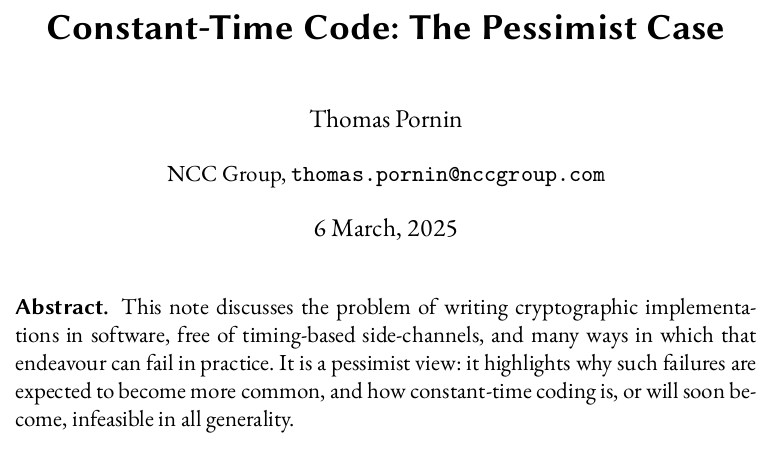
\includegraphics[width=\textwidth]{img/pornin.png}
        \end{column}
    \end{columns}
\end{frame}

\end{document}

